\documentclass{article}

\graphicspath{{/home/david/Book/Chapters/2.Vectors/VectorOperations/pic/}}
% !TeX root = ../../../Mainfile/book.tex



\begin{document}

\color{white}
\subsection{Elementary vector operations}
\color{black}

\begin{align*}
&10 \cdot \irow{3 & 5} & \color{rooj} \textrm{scalar multiplication} \color{black} \\ 
&\irow{3 & 5}^T  & \color{pers} \textrm{transpose} \color{black}\\ 
&\irow{2 & 1} + \irow{1 & 2} &  \color{groen} \textrm{addition}\color{black}\\
&\irow{2 & 1} - \irow{1 & 2} &  \color{blou} \textrm{subtraction}\color{black}
\end{align*}

\paragraph{Operations: } These 4 operations are the most elementary and common operations you will be using in linear algebra. They are 

\begin{itemize}
\item \color{rooj}  Scalar multiplication \color{black} simply multiplies every element of the vector with the scalar
\[
10 \cdot \irow{3 & 5} = \irow{30 & 50}
\]
\item

 \color{pers} Transposing \color{black} a vector is simply converting it from a row-vector to a colum-vector, or a column-vector back to a row-vector
\[
\irow{3 & 5}^T = \icol{3 \\ 5}
\]


\begin{minipage}{0.45\textwidth}
\item \color{groen} Adding \color{black} two vectors is exactly how you would think
\[
\irow{1 & 2} + \irow{2 & 1} = \irow{3  & 3}
\]
\end{minipage} \hfill
\begin{minipage}{0.45\textwidth}
\begin{flushleft}
\begin{figure}[H]
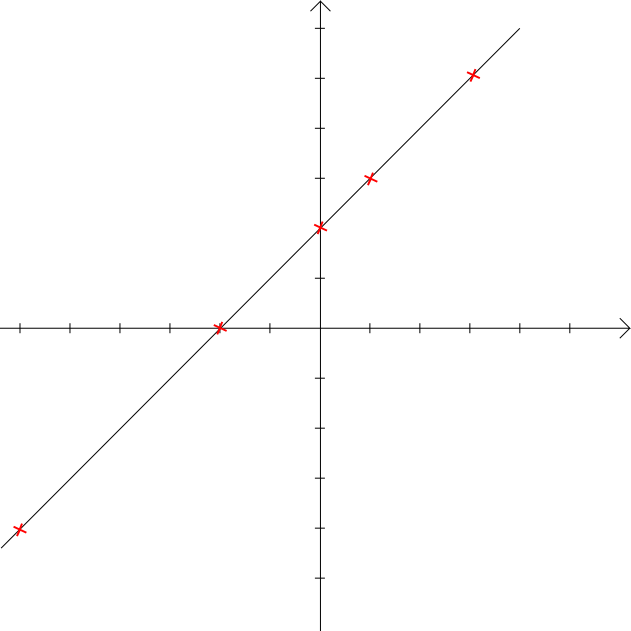
\includegraphics[width = 0.6\linewidth]{1.png}
\end{figure}
\end{flushleft}
\end{minipage}


\begin{minipage}{0.45\textwidth}
\item \color{blou} Subtraction\color{black}, like addition, is just how you'd think
\[
\irow{2 & 1} - \irow{1  & 2} = \irow{1 & -1}
\]

however, drawing subtraction is a bit more involved than addition:
\end{minipage} \hfill
\begin{minipage}{0.45\textwidth}
\begin{flushleft}
\begin{figure}[H]
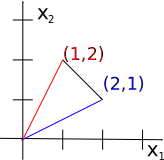
\includegraphics[width = 0.6\linewidth]{2.png}
\end{figure}
\end{flushleft}
\end{minipage}

\end{itemize}

\paragraph{Exercice: } 
Here are 3 vectors, $u = \irow{3 & 5}, v = \irow{8 & 10}, p = \irow{10& 1, 1}$, can you add them together?





\end{document}